In the following, a brief introduction to tensors, tensor networks, and tensor network algorithms is given. We start by defining the conventions and notation used in this thesis in Section \ref{sec:tensors_and_tensor_networks_conventions_and_notation}. In Section \ref{sec:tensors_and_tensor_networks_tensor_decompositions}, we introduce important tensor decompositions that are used extensively in tensor network algorithms. In Section \ref{sec:tensors_and_tensor_networks_isometric_tensor_networks}, we define isometric tensor networks and discuss their properties. Lastly, we give examples for physical states being represented in terms of isometric tensor networks, namely the popular Matrix Product States (MPS) in Section \ref{sec:tensors_and_tensor_networks_matrix_product_states} and the recently developed isometric tensor product states in 2D (isoTPS) in Section \ref{sec:tensors_and_tensor_networks_isometric_tensor_product_states_in_2D}.

\section{Conventions and Notation}
\label{sec:tensors_and_tensor_networks_conventions_and_notation}
For the purpose of this thesis a \textit{tensor} $\bm{T}$ \textit{of rank} $n$ is an $n$-dimensional array of complex numbers
\begin{equation}
	\bm{T} \in \mathbb{C}^{\chi_1\times\chi_2\times\dots\times\chi_n}, \quad \chi_i \in \{1, 2, \dots\}
\end{equation}
with entries
\begin{equation}
	T_{i_1i_2\dots i_n} \in \mathbb{C}, \quad i_j \in \{1, 2, \dots, \chi_j\}.
\end{equation}
\begin{figure}
	\centering
	\includegraphics[width=0.8\textwidth]{figures/Tensor_Networks/basic_tensor_diagrams.jpeg}
	\caption{Tensors of different ranks are shown in diagrammatic notation. (a) A scalar $a\in\mathbb{C}$. (b) A vector $\bm{b}\in\mathbb{C}^{\chi}$. (c) A matrix $\bm{C}\in\mathbb{C}^{\chi_1\times\chi_2}$. (d) A rank-$n$ tensor $\bm{T}\in\mathbb{C}^{\chi_1\times\chi_2\times\dots\times\chi_n}$}.
	\label{fig:basic_tensor_diagrams}
\end{figure}
With this definition, a rank-0 tensor is a scalar, a rank-1 tensor is a vector, and a rank-2 tensor is a matrix. It is convenient to introduce a diagrammatic notation, where tensors are drawn as shapes and tensor indices are drawn as lines (\textit{legs}) emerging from the shapes. To relate this diagrammatic notation to equations, one often decorates each line with the corresponding index $i_j$. A scalar, vector, matrix, and a general rank-$n$ tensor are visualized in this notation in figure \figref{fig:basic_tensor_diagrams}.\par
A \textit{tensor contraction} between two tensors along one or multiple indices is the linear operation that is given by summing over all contracted indices. Given a rank-$(n+f)$ tensor $\bm{X} \in \mathbb{C}^{\chi_1\times\dots\times\chi_n\times\xi_{1}\times\dots\times\xi_{f}}$ and a rank-$(m+f)$ tensor $\bm{Y} \in \mathbb{C}^{\lambda_1\times\dots\times\lambda_m\times\xi_1\times\dots\times\xi_f}$, the result of contracting $\bm{X}$ and $\bm{Y}$ along the last $f$ indices produces a new rank-$(m+n)$ tensor $\bm{Z} \in \mathbb{C}^{\chi_1\times\dots\times\chi_n\times\lambda_1\times\dots\times\lambda_m}$ as
\begin{equation}
	Z_{i_1\dots i_nj_1\dots j_m} \coloneqq \sum_{\alpha_1 = 1}^{\xi_1} \dots \sum_{\alpha_f}^{\xi_f} X_{i_1\dots i_n\alpha_1\dots\alpha_f} Y_{j_1\dots j_n\alpha_1\dots\alpha_f}.
\end{equation}
Arbitrary contractions can be reformulated as contractions over the last $f$ indices by transposing the tensors. By counting the number of multiplications and additions that are necessary to perform the contraction, the computational complexity can be determined as
\begin{equation}
	\label{eq:tensor_contraction_general_computational_complexity}
	\mathcal{O}\left(\prod_{\mu=1}^{n}\chi_\mu \prod_{\mu=1}^{m}\lambda_\mu \prod_{\mu=1}^{f}\xi_f\right).
\end{equation}
A \textit{tensor network} is defined as a collection of tensors that are contracted in a given way. For example, the matrix-vector product of the matrix $\bm{A} \in \mathbb{C}^{\chi_1\times\chi_2}$ and the vector $\bm{b} \in \mathbb{C}^{\chi_2}$ can be written as the contraction of a rank-2 tensor with a rank-1 tensor, resulting in a rank-1 tensor $\bm{b}^\prime \in \mathbb{C}^{\chi_1}$ with entries
\begin{equation}
	\label{eq:example_tensor_network_matrix_vector_product}
	b_i^\prime = \sum_{\alpha=1}^{\chi_2} A_{i\alpha} b_\alpha.
\end{equation}
The matrix product of two matrices $\bm{A} \in \mathbb{C}^{\chi_1\times\chi_2}$ and $\bm{B} \in \mathbb{C}^{\chi_2\times\chi_3}$ can be written as a tensor network of two rank-2 tensors,
\begin{equation}
	\label{eq:example_tensor_network_matrix_product}
	C_{ij} = \sum_{\alpha=1}^{\chi_2} A_{i\alpha} B_{\alpha j},
\end{equation}
where the result is another rank-2 tensor $\bm{C}\in\mathbb{C}^{\chi_1\times\chi_3}$.
As a more involved example we look at a tensor network consisting of two rank-3 tensors $\bm{A}\in\mathbb{C}^{\chi_1\times\chi_2\times\chi_3}$ and $\bm{B}\in\mathbb{C}^{\chi_2\times\chi_4\times\chi_5}$ and one rank-4 tensor $\bm{C}\in\mathbb{C}^{\chi_3\times\chi_5\times\chi_6\times\chi_7}$, where we contract along the dimensions $\chi_2$, $\chi_3$ and $\chi_5$. The result is a rank-4 tensor $\bm{D}\in\mathbb{C}^{\chi_1\times\chi_4\times\chi_6\times\chi_7}$:
\begin{equation}
	\label{eq:example_tensor_network_involved_network}
	D_{ijkl} = \sum_{\alpha=1}^{\chi_2} \sum_{\beta=1}^{\chi_3} \sum_{\gamma=1}^{\chi_5} A_{i \alpha \beta} B_{\alpha j\gamma} C_{\beta \gamma k l}.
\end{equation}
In tensor network diagrams, contractions are visualized by connecting the lines corresponding to contracted indices. In figure \figref{fig:basic_tensor_network_diagrams} we show tensor network diagrams for the tensor networks \eqref{eq:example_tensor_network_matrix_vector_product}, \eqref{eq:example_tensor_network_matrix_product} and \eqref{eq:example_tensor_network_involved_network}. \par
Because tensor contractions are linear, the order in which tensors are contracted doesn't change the result. However, the computational complexity does in general depend on the order of contractions and can thus be minimized by choosing the optimal contraction order.
\begin{figure}
	\centering
	\includegraphics[width=0.8\textwidth]{figures/Tensor_Networks/basic_tensor_network_diagrams.jpeg}
	\caption{Different simple tensor networks are shown in diagrammatic notation. (a) matrix-vector product \eqref{eq:example_tensor_network_matrix_vector_product}. (b) matrix-matrix product \eqref{eq:example_tensor_network_matrix_product}. (c) Tensor network consisting of three tensors \eqref{eq:example_tensor_network_involved_network}.}
	\label{fig:basic_tensor_network_diagrams}
\end{figure}

\newpage
\section{Tensor Decompositions}
\label{sec:tensors_and_tensor_networks_tensor_decompositions}
There are three decompositions that are used extensively in this thesis: The QR-decomposition, the Singular Value Decomposition, and the Polar Decomposition. All three decompositions are matrix decompositions but can be applied to tensors as well by first grouping indices and reshaping to a matrix, applying the decomposition, and reshaping the result back to the original bond dimensions. \par
The \textit{reduced QR-decomposition} of a matrix $\bm{A} \in \mathbb{C}^{n\times m}$ is the decomposition
\begin{equation}
	\label{eq:QR_decomposition_general}
	\bm{A} = \bm{Q}\bm{R},
\end{equation}
where $\bm{Q}\in\mathbb{C}^{n\times k}$ is an isometry, $\bm{R}\in\mathbb{C}^{k\times m}$ is an upper triangular matrix and $k \coloneqq \min(n, m)$. The computational complexity of the QR decomposition scales as
\begin{equation}
	\label{eq:QR_decomposition_complexity}
	\mathcal{O}\left(n\cdot m\cdot\min(n, m)\right).
\end{equation}
A diagrammatic depiction of the QR decomposition \eqref{eq:QR_decomposition_general} is drawn in figure \figref{fig:tensor_decomposition_diagrams}(a). \par
The \textit{Singular Value Decomposition} (SVD) of a matrix $\bm{A} \in \mathbb{C}^{n\times m}$ is the decomposition
\begin{equation}
	\label{eq:SVD_general}
	\bm{A} = \bm{U}\bm{S}\bm{V}^\dagger,
\end{equation}
where $\bm{U}\in\mathbb{C}^{n\times k}$ and $\bm{V}\in\mathbb{C}^{m\times k}$ are isometries, $\bm{S}\in\mathbb{R}^{k\times k}$ is a diagonal real matrix of \textit{singular values}, and $k \coloneqq \min(n, m)$. The computational complexity of the SVD is the same as for the QR decomposition \eqref{eq:QR_decomposition_complexity}. However, while the scaling is the same, the prefactors are lower for the QR decomposition in most implementations, meaning that the QR decomposition is faster in practice. Moreover, in contrast to the SVD, the QR decomposition allows for highly efficient implementations on graphics processing units (GPUs), which enables decompositions of large matrices to be carried out significantly faster and more power efficiently. Thus, whenever the singular values are not needed, the QR decomposition is preferred over the SVD. Figure \figref{fig:tensor_decomposition_diagrams} shows a tensor network diagram of the SVD \eqref{eq:SVD_general}. \par
An important property of the SVD is that it can be used to approximate a matrix $\bm{A}$ by a matrix $\tilde{\bm{A}}$ of lower rank $\chi < \min(m, n)$. This \textit{truncated SVD} can be performed by keeping only the largest $\chi < k$ singular values and omitting the corresponding columns of $\bm{U}$ and $\bm{V}$:
\begin{equation}
	\label{eq:truncated_SVD_general}
	\bm{A} \approx \tilde{\bm{A}} = \tilde{\bm{U}}\tilde{\bm{S}}\tilde{\bm{V}},
\end{equation}
with isometries $\tilde{\bm{U}}\in\mathbb{C}^{n\times\chi}$, $\tilde{\bm{V}}\in\mathbb{C}^{m\times\chi}$ and real diagonal matrix $\tilde{\bm{S}}\in\mathbb{C}^{\chi\times\chi}$. It can be shown \cite{cite:eckart_young_theorem} that the truncated SVD minimizes the distance $\lVert \bm{A} - \bm{\tilde{A}} \rVert_\text{F}$ between $\bm{A}$ and $\tilde{\bm{A}}$ under the constraint $\text{rank}(\tilde{\bm{A}}) = \chi$. The truncated SVD is frequently used in tensor network algorithms to truncate tensors to a maximum bond dimension $\chi_\text{max}$. \par
The \textit{polar decomposition} of a matrix $\bm{A} \in \mathbb{C}^{n\times m}$ is the decomposition
\begin{equation}
	\label{eq:polar_decomposition_general}
	\bm{A} = \bm{W}\bm{P},
\end{equation}
where $\bm{W}\in\mathbb{C}^{m\times n}$ is an isometry and $\bm{P}\in\mathbb{C}^{n\times n}$ is positive-definite and hermitean. The polar decomposition is related to the SVD $\bm{A} = \bm{U}\bm{S}\bm{V}$ by
\begin{equation}
	\label{eq:polar_decomposition_connection_to_svd}
	\bm{W} = \bm{U}\bm{V}^\dagger, \quad \bm{P} = \bm{V}\bm{S}\bm{V}^\dagger.
\end{equation}
The computational complexity of the polar decomposition is the same as for the QR decomposition and SVD \eqref{eq:QR_decomposition_complexity}. The polar decomposition \eqref{eq:polar_decomposition_general} is depicted diagrammatically in figure \figref{fig:tensor_decomposition_diagrams} One can show \todo{prove in appendix?} that the $\bm{W}$ factor of the polar decomposition is the isometry "closest" to the matrix $\bm{A}$, i.e. the isometry that minimizes the distance $\lVert\bm{A}-\bm{W}\rVert_\text{F}$. Thus, the polar decomposition is often used in isometric tensor network algorithms to "isometrize" tensors.
\begin{figure}
	\centering
	\includegraphics[width=0.8\textwidth]{figures/Tensor_Networks/tensor_decomposition_diagrams.jpeg}
	\caption{Different tensor decompositions are shown in tensor network diagram notation. The indices are decorated with bond dimensions. (a) QR decomposition \eqref{eq:QR_decomposition_general}. (b) Singular Value Decomposition \eqref{eq:SVD_general}. (c) Polar decomposition \eqref{eq:polar_decomposition_general}.}
	\label{fig:tensor_decomposition_diagrams}
\end{figure}

\section{Isometric Tensor Networks}
\label{sec:tensors_and_tensor_networks_isometric_tensor_networks}
An isometric tensor network is a tensor network whose tensor diagrams bonds can be consistently assigned with arrows. In particular we will look at finite tensor networks with all arrows pointing to a single tenser, the \textit{orthogonality center}. Such networks have very useful properties, which we will explain in the following.

\newpage
\section{Matrix Product States (MPS)}
\label{sec:tensors_and_tensor_networks_matrix_product_states}
The Density Matrix Renormalization Group (DMRG) algorithm, which was subsequently understood as a variational method over the class of Matrix Product States (MPS), has developed to be the de-facto standard for the numerical simulation of one-dimensional quantum systems. The success of this method is due to the remarkable ability of MPS to capture the area-law entanglement characteristics of ground states of gapped Hamiltonians. Additionally, due to the elegant diagrammatic notation for tensor networks, new algorithms can be developed and discussed efficiently and intuitively. Applications of MPS include finding ground and thermal states, real and imaginary time evolution, and the computation of dynamical properties of lattice Hamiltonians. In the following we give a brief introduction to MPS, for a more in-depth discussion see \cite{cite:DMRG_in_the_age_of_MPS, cite:practical_introduction_MPS_and_PEPS, cite:tenpy}. \par
The state of a quantum many-body system can be written as
\begin{equation}
	\left|\Psi\right\rangle = \sum_{i_1=1}^{d_1} \sum_{i_2=1}^{d_2} \cdots \sum_{i_N=1}^{d_N} \Psi_{i_1i_2\dots i_N} \left|i_1\right\rangle \otimes \left|i_2\right\rangle \otimes \cdots \otimes \left|i_N\right\rangle.
\end{equation}
where N is the number of subsystems (e.g. lattice sites or particles), and $\left\{\left|i_1\right\rangle \otimes \left|i_2\right\rangle \otimes \dots \otimes \left|i_N\right\rangle\right\}$, $i_j = 0, \dots, d_j$ is a set of basis vectors of the full many-body Hilbert space
\begin{equation}
	\mathcal{H} = \bigotimes_{j=1}^{N} \mathcal{H}_j,
\end{equation}
with $\dim\left(\mathcal{H}_j\right) = d_j$ the dimension of the local Hilbert space of subsystem $j$. To simplify the notation, we will assume that the dimension of all local subsystems is the same, $d_j = d$. The $d^N$ complex numbers $\Psi_{i_1i_2\dots i_N}$ fully describe the quantum many-body state, and one can think of $\Psi\in\mathbb{C}^{d\times\cdots\times d}$ as a tensor of rank $N$. However, due to the size of the tensor scaling exponentially with system size, only very small system sizes are accessible computationally. One proceeds by writing $\Psi$ as a tensor network of smaller tensors. A \textit{Matrix Product State} (MPS) is constructed by introducing $N$ rank-3 tensors $A^{[n]}\in\mathbb{C}^{d\times \chi_{n-1}\times \chi_{n}}$ and contracting them in a chain as
\begin{equation}
	\label{eq:MPS_open_boundary_conditions_general_definition}
	\Psi_{i_1i_2\cdots i_N} \coloneqq \sum_{\alpha_1=1}^{\chi_1} \sum_{\alpha_2=1}^{\chi_2}\dots\sum_{\alpha_{N-1}=1}^{\chi_{N-1}}A^{[1],i_1}_{1,\alpha_1} A^{[1],i_2}_{\alpha_1,\alpha_2} \cdots A^{[N],i_N}_{\alpha_{N-1},1},
\end{equation}
where we have written the physical indices $i_n$ as superscripts, such that the sums are performed only over subscripts. Note that in this notation the bond dimensions at the two ends of the chain is $\chi_0 = \chi_{N} = 1$, and we can interpret the tensors $A^{[1]}$ and $A^{[N]}$ as tensors of rank-2. A tensor diagram of the MPS \eqref{eq:MPS_open_boundary_conditions_general_definition} is given in figure \figref{fig:mps_general}.\par
\begin{figure}
	\centering
	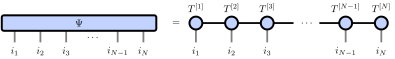
\includegraphics[scale=1]{figures/tikz/Tensor_Networks/mps_basic/mps_basic.pdf}
	\caption{Diagrammatic representation of the Matrix Product State \ref{eq:MPS_open_boundary_conditions_general_definition}.}
	\label{fig:mps_general}
\end{figure}
\begin{figure}
	\centering
	\subcaptionbox{\label{fig:mps_canonical_form_general_definitiom}}
	{%
		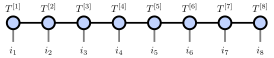
\includegraphics[scale=1]{figures/tikz/Tensor_Networks/mps_canonical_form/mps_canonical_form_a.pdf}
	}
	\subcaptionbox{\label{fig:mps_left_isometry_condition}}
	{%
		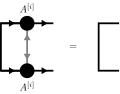
\includegraphics[scale=1]{figures/tikz/Tensor_Networks/mps_canonical_form/mps_canonical_form_b.pdf}
	}
	\quad\quad\quad\quad\quad\quad
	\subcaptionbox{\label{fig:mps_right_isometry_condition}}
	{%
		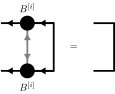
\includegraphics[scale=1]{figures/tikz/Tensor_Networks/mps_canonical_form/mps_canonical_form_c.pdf}
	}
	\caption{(a) Diagrammatic representation of an MPS in canonical form. (b) The isometry condition can be used to simplify contractions.}
	\label{fig:mps_canonical}
\end{figure}
An important property of MPS is the existence of a \textit{canonical form} as an isometric tensor network, where a single tensor $A^{[n]}$ is selected as the orthogonality center. One can bring an arbitrary MPS into this canonical form through successive QR-decompositions or SVDs, starting at the outer ends of the chain and isometrizing one tensor at a time, until the orthogonality center is reached \cite{cite:DMRG_in_the_age_of_MPS}. In figure \figref{fig:mps_canonical}(a) an MPS in canonical with the orthogonality center at subsystem $n$ is visualized in diagrammatic notation. The canonical form greatly simplifies many operations on MPS and allows for the formulation of efficient algorithms, where many contractions reduce to identity due to the isometry condition \eqref{eq:isometry_condition_general}, see also figure \figref{fig:mps_canonical}(b). For example, the expectation value $\left\langle\Psi\right|\hat{O}\left|\Psi\right\rangle$ of a one-site operator $\hat{O} \in \mathbb{C}^{d\times d}$ acting on site $n$ can for a general MPS be computed as
\begin{equation}
\begin{split}
	\label{eq:computation_of_expectation_value_MPS}
	\left\langle\Psi\right|\hat{O}\left|\Psi\right\rangle &=\sum_{i_1,\dots,i_N,j_n=1}^{d}\Psi_{i_1,i_2,\dots,i_N} \Psi_{i_1,\dots,i_{n-1},j_n,i_{n+1},\dots,i_N}^* \left\langle j_n\right|\hat{O} \left|i_n\right\rangle \\
	&= \sum_{i_1,\dots,i_N,j_n=1}^{d} \left(A^{[1],i_1}\cdots A^{[N],i_N}\right) \\
	&\quad\quad\quad\quad\quad\,\,\cdot\left(A^{[1],i_1*}\cdots A^{[N],j_n*} \cdots A^{[N],i_N*}\right)\cdot \hat{O}_{i_n,j_n},
\end{split}
\end{equation}
where the $A^{[n],i_n}$ are interpreted as matrices for $1 < n < N$ and as row/column vectors for $n = 1, N$ such that the product
\begin{equation}
	\left(A^{[1],i_1}\cdots A^{[N],i_N}\right)
\end{equation}
gives a scalar. The contraction \eqref{eq:computation_of_expectation_value_MPS} is visualized as a tensor diagram in figure \figref{fig:mps_local_expectation_value}. Here, the advantage of the diagrammatic notation becomes appearant: It is much easier to understand how tensors are contracted when expressing the contraction in terms of tensor network diagrams. The computational cost of computing the expectation value like this scales linear with the system size $\mathcal{O}\left(N\chi^3d\right)$, where $\chi$ is the maximum virtual bond dimension $\chi = \max\left\{\chi_1,\dots,\chi_N\right\}$. If the MPS is however given in canonical form with the orthogonality center at site $n$, the computation reduces to a contraction of only three tensors as can be seen in figure \figref{fig:mps_local_expectation_value_canonical}, and the computational cost $\mathcal{O}\left(\chi^3d\right)$ becomes independent of system size. \par
\begin{figure}
	\centering
	\includegraphics[scale=1]{figures/tikz/Tensor_Networks/mps_local_expectation_value/mps_local_expectation_value.pdf}
	\caption{The computation of the expectation value of a local operator can be computed by contracting the MPS with its conjugate transpose, with the operator "sandwiched" between.}
	\label{fig:mps_local_expectation_value}
\end{figure}
\begin{figure}
	\centering
	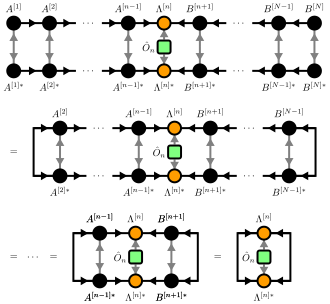
\includegraphics[scale=1.0]{figures/tikz/Tensor_Networks/mps_canonical_form_local_expectation_value/mps_canonical_form_local_expectation_value.pdf}
	\caption{If the MPS is in canonical form, the computation of the expectation value of a local operator can be simplified to a contraction of three tensors using the isometry condition.}
	\label{fig:mps_local_expectation_value_canonical}
\end{figure}
Until now, the MPS representation of $\left|\Psi\right\rangle$ is still exact. One can approximate a MPS by restricting the virtual bond dimension to a maximal bond dimension $\chi_n < \chi_\text{max}$. In this case, the number of parameters that need to be stored to describe the state is reduced from $\mathcal{O}\left(d^N\right)$ to $\mathcal{O}\left(N\chi_\text{max}^2 d\right)$. To arrive at this approximation, two neighbouring tensors can be contracted and split via a truncated SVD, keeping only the $\chi_\text{max}$ largest singular values. If the orthogonality center of the MPS is at one of the two tensors, this approximation is globally optimal as explained in section \ref{sec:tensors_and_tensor_networks_isometric_tensor_networks}. Additionally, this SVD at the orthogonality center is related to the Schimdt decomposition of a bipartite system
\begin{equation}
	\left|\Psi\right\rangle = \sum_{\alpha=1}^{\chi_n} \lambda_\alpha \left| \Psi^{[L]}_\alpha\right\rangle \otimes \left|\Psi^{[R]}_\alpha\right\rangle,
\end{equation}
where the chain is split into a left and right subsystem with orthogonal basis vectors $\left|\Psi^{[L]}_\alpha\right\rangle$ and $\left|\Psi^{[R]}_\alpha\right\rangle$ as visualized in figure \ref{fig}. In this case, the Schmidt values $\lambda_\alpha >= 0$ coincide with the singular values! One can further use this to compute the Von-Neumann entanglement entropy
\begin{equation}
	S = -\sum_{\alpha=1}^{\chi_n} \lambda_\alpha^2 \log\left(\lambda_\alpha^2\right),
\end{equation}
quantifying the amount of entanglement between the left and right subsystems. If the state is normalized, it additionally holds
\begin{equation}
	\sum_{\alpha=1}^{\chi_n} \lambda_\alpha^2 = 1.
\end{equation}
Thus, how well an MPS of a given bond dimension $\chi_\text{max}$ is able to represent a given quantum state is highly dependent on the Schmidt spectrum $\left\{\lambda_\alpha\right\}$ at the different bipartitions of the chain. If the Schmidt values decrease exponentially, only an exponentially small part of the entanglement structure is truncated and the truncated MPS is a good approximation for the original state. It can be shown \cite{cite:area_law_1D_proof, cite:area_laws_review} that for ground states of local, gapped, one dimensional Hamiltonians there holds an \textit{area law}: The entanglement entropy at arbitrary bipartitions of the chain is bounded by a constant
\begin{equation}
	S \le S_\text{max}, 
\end{equation}
where $S_\text{max}$ is independent of the system size. This is in contrast to the fact that the entanglement of states drawn randomly from the many-body Hilbert space on average exhibits \textit{volume law} scaling
\begin{equation}
	\mathbb{E}\left[S\right] > \min\left(N_L, N_R\right)\log(d),
\end{equation}
where $N_L$ and $N_R$ are the number of subsystems in the left and right bipartition. Hence, ground states of gapped Hamiltonians are very nongeneric. Note that the constant $S_\text{max}$ scales with the correlation length of the system, which diverges when approaching critical points. \par
It is immediately clear that truncated MPS by construction exhibit area law entanglement scaling, if the local subsystems that are represented by each tensor correspond to physical systems on a 1D chain. The maximal entanglement entropy for a bipartition can be reached when all Schmidt values are equal, $\lambda_\alpha = 1/\sqrt{\chi_n}$, and thus
\begin{equation}
	S \le \log\left(\chi_\text{max}\right)
\end{equation}
for arbitrary bipartitions of the chain. One can conclude that MPS are good approximations for ground states of gapped 1D Hamiltonians away from criticality. \par 
For completeness we note that the truncation of all bonds of an MPS is a highly non-linear optimization problem and the naive algorithm of truncating each bond with an SVD does in general not lead to a minimal error. A variational compression procedure can often be used to obtain a lower error at the same maximum bond dimension $\chi_\text{max}$ \cite{cite:DMRG_in_the_age_of_MPS}.
\par
Many algorithms have been formulated in the language of MPS. Most notably, the Density Matrix Renormalization Group (DMRG) algorithm can be used for finding ground states of local lattice Hamiltonians \cite{cite:DMRG_in_the_age_of_MPS}. Time evolution of MPS can be performed with the the Time Evolving Block Decimation (TEBD) algorithm \cite{cite:efficient_simulation_of_1D_quantum_many_body_systems, cite:matrix_product_density_operators_simulation_of_finite_temperature_and_dissipative_systems} or the Time Dependant Variational Principle (TDVP) \cite{cite:time_dependent_variational_principle_for_quantum_lattices, cite:unifying_time_evolution_and_optimization_with_MPS}. In the following, we will briefly discuss TEBD, as the algorithm can be generalized easily to isometric tensor product states of higher dimension, which we will do in section \ref{} \todo{Add ref}. \par
Assume that we are given a quantum state $\left|\Psi\right\rangle$ in the form of an MPS and a Hamiltonian $\hat{H}$ that can be written as a sum of nearest-neighbour operators $\hat{h}_{j,j+1}$,
\begin{equation}
	\hat{H} = \sum_{j = 1}^{N-1} \hat{h}^{[j,j+1]}.
\end{equation}
The state $\left|\Psi\right\rangle$ can be evolved in time as
\begin{equation}
	\left|\Psi(t)\right\rangle = \hat{U}\left(t\right) \left|\Psi\right\rangle = e^{-it\hat{H}} \left|\Psi\right\rangle,
\end{equation}
where we set $\hbar = 1$. The time evolution operator $U(t)$ is in general very hard to compute and handle exactly. Thus, $U(t)$ is approximated using a Suzuki-Trotter decomposition. We start by decomposing the time evolution into a series of $K$ small time steps $\Delta t = t/K$ as
\begin{equation}
	U(t) = e^{-it\hat{H}} = \left(e^{-i\Delta t\hat{H}}\right)^K = \left(U(\Delta t)\right)^K.
\end{equation}
Next, we split the Hamiltonian into terms acting on even and odd bonds
\begin{equation}
	\hat{H} = \sum_{j \text{ even}}\hat{h}^{[j, j+1]} + \sum_{j \text{ odd}}\hat{h}^{[j, j+1]} \eqqcolon H_\text{even} + H_\text{odd}.
\end{equation}
Using the Baker-Campbell-Hausdorff formula we can then approximate
\begin{equation}
	\begin{split}
		U(\Delta t) &= e^{-i\Delta t\left(H_\text{even} + H_\text{odd}\right)} = e^{-i\Delta tH_\text{even}}e^{-i\Delta tH_\text{odd}}e^{-i\Delta t^2\left[H_\text{even}, H_\text{odd}\right]}\\
		&= e^{-i\Delta tH_\text{even}}e^{-i\Delta tH_\text{odd}} + \mathcal{O}\left(\Delta t^2\right) = \hat{U}^\text{TEBD1}(\Delta t) + \mathcal{O}\left(\Delta t^2\right),
	\end{split}
\end{equation}
which is called a Suzuki-Trotter decomposition of first order. Since operators acting on even bonds commute with operators acting on other even bonds, the exponentials $e^{-i\Delta tH_\text{even}}$ and $e^{-i\Delta tH_\text{odd}}$ factorize,
\begin{equation}
	e^{-i\Delta tH_\text{even}} = e^{-i\Delta t\sum_{j \text{ even}} h^{[j, j+1]}} = \prod_{j \text{ even}} e^{-i\Delta t h^{[j, j+1]}}.
\end{equation}
Each bond operator $e^{-i\Delta t h^{[j, j+1]}}$ acting on the combined Hilbert space of sites $j$ and $j+1$ can be reshaped into a tensor of rank 4. The application of the operator $\hat{U}^\text{TEBD1}(\Delta t)$ to a state in MPS form can thus be written as the tensor network in figure \ref{}.
To perform a single TEBD iteration corresponding to a time evolution of $\Delta t$ we want to approximate this tensor network by a new MPS. This can be done by moving the orthogonality center from left to right, applying the bond operators $e^{-i\Delta t h^{[j, j+1]}}$ while keeping the MPS structure. The process of applying a single bond operator is shown in figure \ref{}. First, the two site tensors and $e^{-i\Delta t h^{[j, j+1]}}$  are contracted into a single tensor, that is then split and truncated again using an SVD. By sweeping twice across the MPS, first applying the bond operators on all even bonds and then the bond operators on all odd bonds, we perform a full TEBD iteration. There exist two sources of errors, the truncation error of the truncated SVD and the error of the Suzuki-Trotter decomposition. The truncation error can be controlled by choosing a larger bond dimension $\chi$, allowing the representation of more entanglement and thus the evolution to larger times. However, generally the amount of entanglement grows exponentially in time, necessitating an exponentially growing bond dimension and practically limiting the algorithm to small times. A smaller Suzuki-Trotter error can be achieved by choosing higher-order Suzuki-Trotter decomposition. For example, a second order decomposition can be computed as
\begin{equation}
	\begin{split}
		U(\Delta t) &= e^{-i\Delta t\left(H_\text{even} + H_\text{odd}\right)} = e^{-i\frac{\Delta t}{2}H_\text{even}} e^{-i\Delta t H_\text{odd}} e^{-i\frac{\Delta t}{2}H_\text{even}} + \mathcal{O}\left(\Delta t^3\right)\\
		&= \hat{U}^\text{TEBD2}(\Delta t) + \mathcal{O}\left(\Delta t^3\right).
	\end{split}
\end{equation}
\todo{Discuss different method of 2nd order tebd (ladder vs chain)}
Higher order Suzuki-Trotter decompositions are also possible \cite{cite:finding_exponential_product_formulas_of_higher_orders}.

\section{Isometric Tensor Product States in 2D}
\label{sec:tensors_and_tensor_networks_isometric_tensor_product_states_in_2D}
The natural generalization of MPS to higher dimensional lattices is given by \textit{Projected Entangled Pair States} (PEPS). A PEPS is constructed similar to a MPS by representing the local subsystem on each lattice site $i$ with the index $\sigma_i$ of a tensor $T_i^{\sigma_i}$ and connecting nearest-neighbour tensors with virtual bonds. The quantum state can then be written as
\begin{equation}
	\label{eq:PEPS_definition_general}
	\left|\Psi\right\rangle = \sum_{\sigma_1,\sigma_2,\dots,\sigma_N} \mathcal{C}\left(T_1^{\sigma_1}, T_2^{\sigma_2}, \dots, T_N^{\sigma_N}\right) \left|\sigma_1,\sigma_2,\dots,\sigma_N\right\rangle,
\end{equation}
where $\mathcal{C}(\dots)$ denotes the contraction of the full network along all virtual bonds. As an example, we draw a PEPS on a square lattice in figure \figref{fig:square_PEPS}. \par
\begin{figure}
	\centering
	\subcaptionbox{\label{fig:square_PEPS}}
	{%
		\includegraphics[scale=1]{figures/tikz/Tensor_Networks/isoTPS_structure/isoTPS_structure_a.pdf}
	}
	\quad\quad
	\subcaptionbox{\label{fig:square_isoTPS}}
	{%
		\includegraphics[scale=1]{figures/tikz/Tensor_Networks/isoTPS_structure/isoTPS_structure_b.pdf}
	}
	\caption{Tensor Networks representing two dimensional states on a square lattice. (a) A Projected Entangled Pair State (PEPS). (b) An isometric Tensor Product State (isoTPS). \todo{Include orthogonality center tensor}}
	\label{fig:square_PEPS_and_isoTPS}
\end{figure}
PEPS are able to efficiently represent area-law states in two and higher dimensions \cite{cite:practical_introduction_MPS_and_PEPS}. Remarkably, PEPS can even handle correlations decaying polynomially with separation distance \cite{cite:criticality_the_area_law_and_the_computational_power_of_PEPS}, whereas MPS can only handle exponentially decaying correlations. Polynomially decaying correlations are characteristic for critical points. \par
Unfortunately, it is not generally possible to bring a PEPS into an exact canonical form due to the presence of closed loops. Thus, already the computation of local expectation values scales exponentially with system size and can in practice be only done approximately, e.g. using the boundary MPS method \cite{cite:practical_introduction_MPS_and_PEPS} or corner transfer matrices \cite{cite:CTMRG}. Moreover, algorithms for ground state search and time evolution have computational costs scaling with high powers of the bond dimension. For example the cost of a full update TEBD or DMRG iteration is dominated by the contraction of an effective environment, scaling as $\mathcal{O}\left(D^{10}\right)$ \cite{cite:unifying_PEPS_contractions}. \par
Recently, the new class of \textit{isometric Tensor Product States} (isoTPS) has been introduced \cite{cite:isometric_tensor_network_states_in_two_dimensions, cite:conversion_of_PEPS_into_a_canonical_form, cite:DMRG_approach_to_optimizing_2D_tensor_networks}, generalizing the canonical form of MPS to higher dimensions by enforcing isometry constraints. This allows for efficient computation of local expectation values and greatly lowers the cost of some algorithms. The downside to this approach is that the set of states representable by isoTPS is smaller than the set of state representable by PEPS. It is thus an interesting question to ask which kinds of states and, more generally, which kinds of quantum phases can still be represented by isoTPS. \par
In the following, we will give a brief introduction to the isoTPS defined in \cite{cite:isometric_tensor_network_states_in_two_dimensions} and discuss their properties. A two-dimensional isoTPS on the square lattice is constructed by enforcing the isometry conditions shown in figure \figref{fig:square_isoTPS}. All isometries are chosen in such a way that all arrows point towards a special row and column, called the \textit{orthogonality hypersurface} of the isoTPS. The term "hypersurface" is chosen in anticipation of a generalization to higher dimensions. Because of the isometry condition, one can think of the contractions of each of the four regions outside the orthogonality hypersurface as orthogonal boundary maps \cite{cite:efficient_simulation_of_dynamics_in_two_dimensional_quantum_spin_systems}. The single tensor with only incoming arrows is called the \textit{orthogonality center}. local expectation values of operators acting in the vicinity of the orthogonality center can be computed efficiently because most contractions reduce to identity, similar to the computation of local expectation values in MPS (see figure \figref{fig:mps_local_expectation_value_canonical}). The orthogonality center can be moved along the orthogonality hypersurface simply and exactly using a QR-decomposition as shown in figure \figref{fig:isoTPS_moving_ortho_center}. \par
\begin{figure}
	\centering
	\includegraphics[scale=1]{figures/tikz/Tensor_Networks/isoTPS_moving_ortho_center/isoTPS_moving_ortho_center.pdf}
	\caption{Moving the orthogonality center and the orthogonality hyper surface around is a central problem in isoTPS applications. (a) Moving the orthogonality center along the orthogonality hypersurface can be done easily via QR-decompositions. (b) An orthogonality column can be moved by first solving equation \eqref{eq:isoTPS_moving_ortho_surface_auxillary_formulation} variationally and then absorbing $\Lambda$ into $B_{l+1}$ via the standard MPO-MPS multiplication and MPS compression algorithms.}
	\label{fig:isoTPS_moving_ortho_center}
\end{figure}
\begin{figure}
	\centering
	\includegraphics[scale=1]{figures/tikz/Tensor_Networks/isoTPS_moving_ortho_surface/isoTPS_moving_ortho_surface.pdf}
	\caption{The orthogonality hypersurface can be moved to the right by first solving equation \eqref{eq:isoTPS_moving_ortho_surface_auxillary_formulation} variationally and then absorbing $\Lambda$ into $B^{[n+1]}$ via the standard MPO-MPS multiplication and MPS compression algorithms.}
	\label{fig:isoTPS_moving_ortho_column}
\end{figure}
Moving the orthogonality surface is a harder problem, which in general can only be done approximately. In analogy to MPS and as shown in figure \figref{fig:square_isoTPS}, we call columns left of the orthogonality hypersurface $A_l$ and tensors right of the orthogonality hypersurface $B_l$, with $l = 1,2,\dots,L$ and $L$ the linear system size. Moving the orthogonality hypersurface $\Lambda_l$ one column to the right can be expressed as solving the problem
\begin{equation}
	\label{eq:isoTPS_moving_ortho_surface_general}
	\Lambda_l B_{l+1} = A_l \Lambda_{l+1},
\end{equation}
where the notation $\Lambda_l B_{l+1}$ means the contraction of columns $\Lambda_l$ and $B_{l+1}$ along their connecting bonds. Instead of \eqref{eq:isoTPS_moving_ortho_surface_general}, one can solve the simpler auxillary problem
\begin{equation}
	\label{eq:isoTPS_moving_ortho_surface_auxillary_formulation}
	\Lambda_l = A^l \Lambda,
\end{equation}
where $\Lambda$ is a column of tensors with no physical indices, as shown in figure \figref{fig:isoTPS_moving_ortho_column}. This column can then be absorbed into $B_{l+1}$ via the standard algorithm of applying an MPO to an MPS and subsequent MPS compression \cite{cite:DMRG_in_the_age_of_MPS}. One can variationally solve problem \eqref{eq:isoTPS_moving_ortho_surface_auxillary_formulation} by minimizing the distance $\left\lvert\Lambda_l-A_l\Lambda\right\rvert$, sweeping back and forth through the tensors while respecting the isometry condition.\todo{Maybe reference Evenbly-Vidal here?}
\begin{figure}
	\centering
	\subcaptionbox{\label{fig:Moses_move}}
	{%
		\includegraphics[scale=1]{figures/tikz/Tensor_Networks/isoTPS_MM/isoTPS_MM_a.pdf}
	}
	\subcaptionbox{\label{fig:tripartite_decomposition}}
	{%
		\includegraphics[scale=1]{figures/tikz/Tensor_Networks/isoTPS_MM/isoTPS_MM_b.pdf}
		
	}
	\caption{(a) The Moses Move (MM) splits the column $\Lambda_l$ into $A_l$ and $\Lambda$ via a single unzipping sweep of tripartite decompositions. (b) Tripartite decomposition of the tensor $W$ as explained in the text.}
	\label{fig:Moses_move_and_tripartite_decomposition}
\end{figure}
It is however found in \cite{cite:isometric_tensor_network_states_in_two_dimensions} that a single unzipping sweep, called the \textit{Moses Move} (MM), provides a solution very close to the variational one whilst being far quicker. The MM can also be used as a good initialization for the variational algorithm. We sketch the MM in figure \figref{fig:Moses_move}. We start from the bottom of the orthogonality hypersurface column and split the tensors one after the other using a tripartite decomposition. A single tripartite decomposition of a tensor $W$ is shown in figure \figref{fig:tripartite_decomposition}. First, $W$ is split into two tensors $A$ and $B$ via a truncated SVD $W = U(SV) = AB$ with $A$ an isometry. The bond connecting A and B is reshaped into two bonds. Next, it is important to note that the full contraction is invariant under the insertion of a unitary and its conjugate transpose, $AB = (AU^\dagger)(UB)$, with $(AU^\dagger)$ still satisfying the isometry condition. This degree of freedom can be used to \textit{disentangle} the tensor $B$ along the direction of the red bonds. Accordingly, we choose $U$ such that the truncation error or some entanglement measure is minimized for splits along the direction of the red bonds. Choosing a good disentangling unitary is crucial for a successful tripartite decomposition and will be discussed further in section \ref{sec:}. Assume for now that a good disentangling unitary has been found. After contracting $(AU^\dagger)$ and $(UB)$, a truncated SVD is used to split $(UB)$ into tensors $B^\prime$ and $C^\prime$ as shown in figure \figref{fig:tripartite_decomposition}, completing the tripartite decomposition. \par
Because the orthogonality center can be moved easily along the orthogonality hypersurface, one can think of the orthogonality hypersurface along a column or row as a 1D MPS with an enlarged physical bond dimension grouping together the phsical and the two ancilla legs pertruding from the orthogonality hypersurface tensors. Standard MPS algorithms can then be generalized to isoTPS by performing one iteration of the algorithm on the orthogonality hypersurface MPS, before moving the hypersurface via MM or variational optimization and repeating the procedure. As an example, we will discuss TEBD$^2$, the generalization of $TEBD$ to an isoTPS on a 2D square lattice. \todo{write}. \par
isoTPS are a new class of states that enable the implementation of faster algorithms for e.g. ground state search and time evolution, compared to PEPS. The expressional power of isoTPS has been studied in \cite{cite:isometric_tensor_network_representation_of_string_net_liquids}, where it was found that isoTPS with finite bond dimension can exactly represent ground state wavefunctions of string-net liquid models, showing that long-range entanglement does not form an obstruction for isoTPS representations and suggesting that the ground states of gapped Hamiltonians with gappable edges can be efficiently represented as an isoTPS. There have also been works discussing the computational complexity of isoTNS \cite{cite:computational_complexity_of_isometric_tensor_network_states} and relating isoTNS to quantum circuits \cite{cite:sequential_generation_of_projected_entangled_pair_states, cite:quantum_circuits_for_2D_isometric_tensor_networks}. In \cite{cite:topological_quantum_phase_transitions_in_2D_isometric_tensor_networks}, topological phase transitions were studied with isoTPS, showing that isoTPS can represent some critical states with power-law correlations. A DMRG$^2$-algorithm was implemented on isoTPS in \cite{cite:efficient_simulation_of_dynamics_in_two_dimensional_quantum_spin_systems} and used to compute dynamical structure factors of ground states using real time evolution. IsoTPS were also extended to fermionic systems \cite{cite:fermionic_isometric_tensor_network_states}, to two dimensional strips of infinite length \cite{cite:two_dimensional_isometric_tensor_networks_on_infinite_strip}, and to three dimensional cubic lattices \cite{cite:three_dimensional_isometric_tensor_networks}. They have also been used to compute properties of two dimensional thermal states \cite{cite:isometric_tensor_network_representation_of_2D_thermal_states}.